\chapter{Introdução}

As metodologias ágeis vem ganhando cada vez espaço no mercado global 
de desenvolvimento de software, pois enfatizam a qualidade do produto 
sobre a qualidade do processo, procurando minimizar a execução 
de atividades não essenciais ao longo do ciclo de vida de 
desenvolvimento de software. 

O eXtreme Programming (XP), que é uma metodologia ágil, tem a codificação como a atividade chave durante um projeto de software \cite{beck1999}. Isso também se torna perceptível por algumas práticas do XP~\footnote{\url{http://www.extremeprogramming.org/}} :

\begin{enumerate}
\item Padronização do Código: O código é a principal forma de comunicação entre a equipe, logo a padronização de código o torna consistente e fácil para todo o time ler e refatorar. 
\item Propriedade Coletiva do Código: Cada programador pode melhorar qualquer parte do código quando existir a oportunidade.
\item Programação em Pares: Todo código é escrito com duas pessoas: uma que olha para uma máquina, e outra com um teclado e um mouse.
\item Integração Contínua: Todo novo código é integrado ao sistema e quando integrado, o sistema é totalmente reconstruído do zero e todos os testes devem passar ou o novo código é descartado.
\end{enumerate} 


Logo em metodologias ágeis, é possível inferir a qualidade do trabalho desenvolvido, por meio do código-fonte. Um dos métodos mais utilizados é a análise estática de código, o qual segundo \citeonline{Emanuelsson2008} significa método automático de coleta de propriedades de tempo de execução do código-fonte sem executá-lo e os resultados da análise podem servir para propósitos de verificação de erros, geração automática de casos de teste, análise de impacto ou ainda para obtenção de métricas de código-fonte.

Embora a definição formal da análise estática consolidada no âmbito acâdemico, vide os trabalhos de \cite{Wichmann95} e \cite{Nielson:1999}, as ferramentas dísponiveis no mercado, que realizam as coletas e avaliação, ainda não suprem totalmente as necessidades de quem precisa avaliar a qualidade total do produto.

Cada ferramenta apresenta suas vantagens e limitações, contudo, de maneira geral é possível citar como limitações das ferramentas de análise estática de código:

\begin{enumerate}
\item Ausência de resultados consolidados do produto, pois não são feitas correlações entre as análises de elementos internos do código fonte (Bibliotecas, Pacotes, Classes, Métodos, Funções).
\item Ausência de mecanismos de tratamento, separação e organização de dados históricos das métricas.
\item Ausência de avaliações qualitativas sobre os valores obtidos para cada métrica, deixando assim a interpretação dos resultados restrita apenas ao nível técnico.
\item Apresentação dos dados não é visualmente agradável.
\item Grande complexidade em sua utilização.
\end{enumerate}


%------------------------------------------------------------------------------%


%------------------------------------------------------------------------------%



%------------------------------------------------------------------------------%

\section{Objetivos}

Esta seção apresenta os objetivos gerais e específicos deste TCC.

\subsection{Objetivos Gerais}
Sob prisma da avaliação da qualidade de código em ambientes ágeis, neste trabalho, há como objetivo geral a proposição e construção um ambiente de \textit{Dwing}, de modo a melhorar extração e visualização das métricas de código-fonte, suprimindo os pontos fracos enunciados acima das ferramentas de análise estática de código.

Este ambiente inicialmente construído para este trabalho de conclusão de curso, poderá aumentado em trabalhos futuros para a correlação de outras métricas coletadas
durante o processo de desenvolvimento de software. 


%------------------------------------------------------------------------------%

\subsection{Específicos}

Os objetivos específicos desse trabalho são:

\begin{enumerate}
	
\item Construir o ambiente de Dwing para métricas de código-fonte.
\item Validar o ambiente com o estudo de caso baseado na abordagem desenvolvida por \citeonline{Meirelles2013}.
\item Incorporar visões gerenciais das métricas de código-fonte.
\item Facilitar o entendimento das métricas de código-fonte.

\end{enumerate}

%------------------------------------------------------------------------------%

\section{Sobre o Trabalho}

\subsection{Cronograma}
O Trabalho de Conclusão de Curso foi planejado, como um planejamento de longo prazo, em quatro ciclos de desenvolvimento de vinte e um dias. As figuras \ref{cronograma} e \ref{gantt}, que foram extraídas do OpenProj\footnote{\url{http://sourceforge.net/projects/openproj/}}, apresentam o cronograma geral o gráfico de Gantt do presente trabalho.

	\begin{figure}[h]
		\centering
			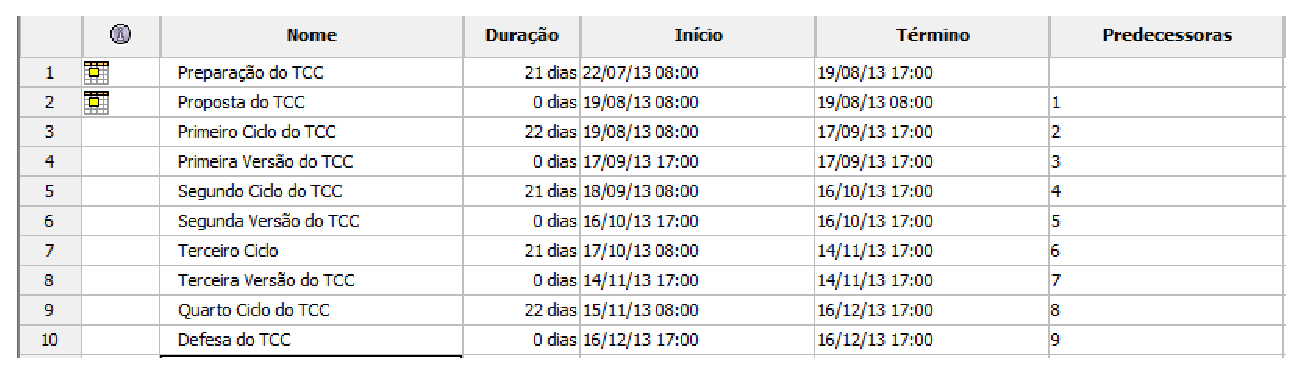
\includegraphics[keepaspectratio=true,scale=0.7]{figuras/calendario_marcos.eps}
		\caption{Ciclos de Desenvolvimento do Trabalho de Conclusão de Curso}
		\label{cronograma}
	\end{figure}

	\begin{figure}[h]
		\centering
			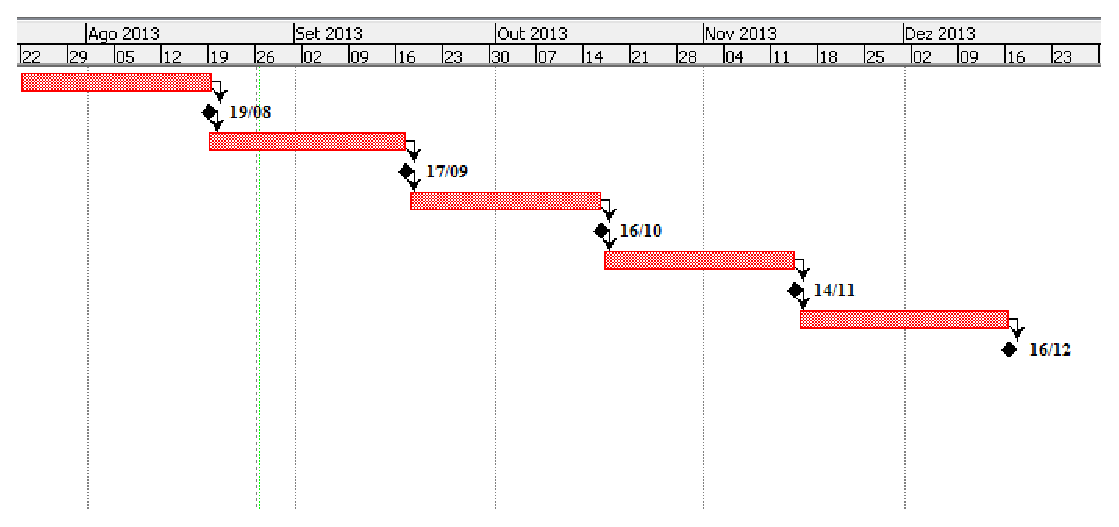
\includegraphics[keepaspectratio=true,scale=0.7]{figuras/gantt_chart.eps}
		\caption{Gráfico de Gantt}
		\label{gantt}
	\end{figure}

Para cada ciclo de desenvolvimento do Trabalho de Conclusão de Curso,  utilizou-se o Quadro \textit{Kanban}  

\subsection {Metodologia de Pesquisa}
Durante a fase inicial do trabalho de conclusão de curso, a metodologia da pesquisa foi definida em pesquisa exploratória, dado que se buscava evidenciar e caracterizar o problema da visualização das métricas obtidas diretamente do código-fonte , 
e pesquisa biblográfica, dada a necessidade de fundamentação teórica sobre cada um dos elementos que compõem o ambiente da solução proposta. Durante a fase de construção do ambiente, utilizou-se
as práticas ágeis como a realização de ciclos curtos e a integração contínua de novos pedaços da solução proposta. Nesta fase, visou-se ainda a aplicação do ambiente em um estudo de caso, 
de forma a  a validar o ambiente proposto.  

\subsection{Organização do Trabalho}
Para a primeira fase deste Trabalho de Conclusão de Curso, além desta introdução
este texto está organizado em capítulos. O Capítulo 2 apresenta a fundamentação teórica
sobre métricas e traz também as métricas de código-fonte, seus intervalos e definições para extração e visualização. O Capítulo 3 apresenta o SonarQube como a ferramenta escolhida para extração das métricas de código-fonte.
O Capítulo 4 apresenta a fundamentação teórica do ambiente de Dwing, de modo a suprir as limitações das ferramentas, e cada um de seus componentes em detalhes. 
O Capítulo 5 apresenta o ambiente proposto por este trabalho para extração e visualização das métricas de código-fonte. Por fim, o Capítulo 6 apresenta o estado atual da validação 
do ambiente por meio de estudo de caso, bem como as atividades planejadas até o encerramento do trabalho de conclusão de curso.
%

